\section{Background}
\label{sec:background}

\begin{figure}[t]
\centering
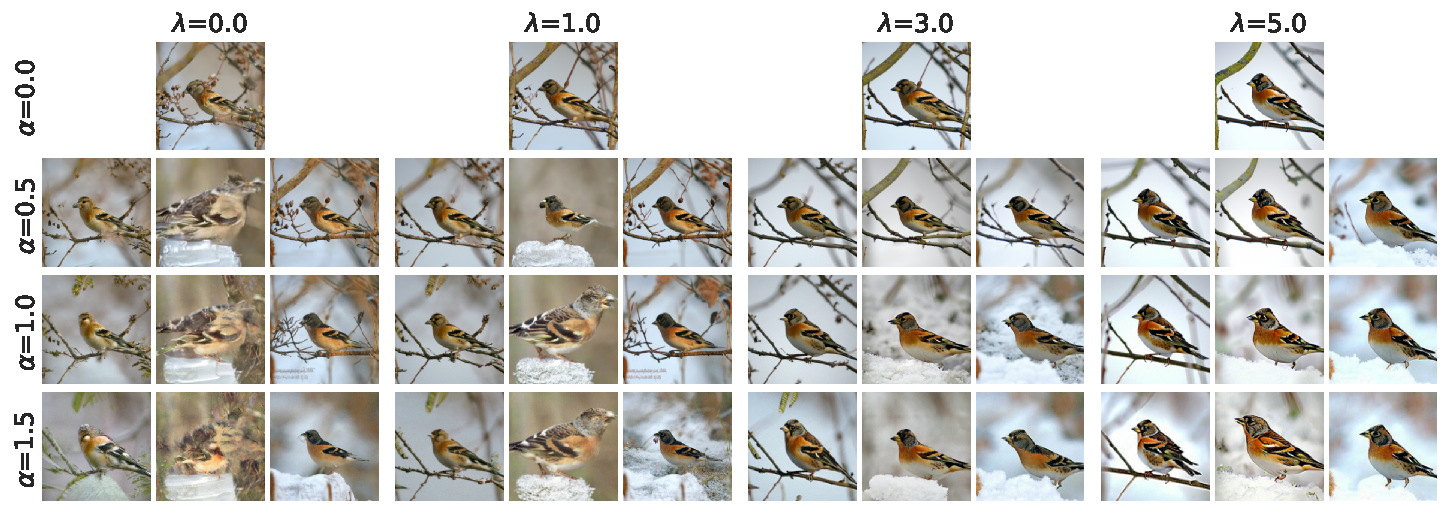
\includegraphics[width=0.99\textwidth]{figs/teaser8.pdf}
\caption{%
    \textbf{Stochastic sampling improves diversity at all classifier-free guidance levels.}
    We visualize samples from a rectified flow model at four classifier-free guidance levels $\lambda$ (\cref{sec:score_function}) and at four stochasticity scales $\alpha$ for NonSingular (\cref{tab:sde_family_table}). 
    Three samples are shown for each configuration where the sampling starts at the same draw from $p_1(x_1)$.
    When $\alpha=0$, the sampler is deterministic and samples are the same (therefore we show only one).
    When $\lambda=0$, there is no classifier-free guidance.
    Note the increased diversity as $\alpha$ increases. More examples in \cref{fig:qual_alpha_vs_lambda}.
}
\label{fig:imagenet_cfg}
\vspace{-0.4cm}
\end{figure}

\paragraph{Notation.}
Throughout this work we use small Latin letters $t, x, y$ etc. to represent scalar and vector variables, $f, g$ etc. to represent functions, Greek letters $\alpha, \beta$ etc. to represent (hyper-)parameters, and capital letters $G$ to represent matrices.
With a slight abuse of notation we use lower case letters $x$ to represent both the random variable and a particular value $x \sim p(x)$.
Whenever unambiguous, we suppress the dependence of state $x_t$ on time $t$ as $x \equiv x_t$, and dependence of functions on state $x_t$ and time $t$ as $f \equiv f(x_t, t)$ to simplify notation.

We briefly discuss rectified flow and continuous time diffusion models.
Refer to \cite{liu2022flow, song2020score} for details.

\subsection{Rectified Flow}
\label{sec:rect_flow}

Let $x_0 \sim p_0(x_0) \in \R^d$ be the draws from the data distribution $p_0$ that we are interested in learning and sampling from.
Let $x_1\sim p_1(x_1) \in \R^d$ be an easy to sample source distribution.
Loosely, the key idea behind the diffusion and flow family of models is to learn a mapping that either stochastically or deterministically transforms a sample from $p_1$, in an iterative manner, to produce a sample from $p_0$.
Let $\nu(x_0, x_1)$ be an arbitrary coupling distribution for the two random variables $x_0, x_1$ such that $p_0(x_0) = \int \nu(x_0, x_1)dx_1, p_1(x_1) = \int \nu(x_0, x_1)dx_0$.
A simple choice is the product of the two: $\nu(x_0, x_1) \equiv p_0(x_0)p_1(x_1)$.
To construct a rectified flow first an interpolation between the two variables is defined as $x_t \equiv h(x_0, x_1, t)$ that is differentiable w.r.t. time.
The default interpolation proposed and studied in \citet{liu2022flow} is:
\begin{equation}
\label{eq:rect_flow_default_interp}
x_t = (1-t)x_0 + t x_1, \quad t \in [0, 1].
\end{equation}
With the above, rectified flow learns a vector field $v(x_t, t)$ by minimizing the following objective:
\begin{equation}
\label{eq:rectflow_obj}
v(x, t) = \argmin_{v'} \mathbb E_{(x_0, x_1)\sim \nu} \left[ \int_0^1 \left\lVert \frac{dx_t}{dt} - v'(x_t, t) \right\rVert^2 dt \right].
\end{equation}
The solution to the above optimization problem is $v(x, t) \equiv \mathbb E[x_1 - x_0 |x,t]$ and is referred to as 1-Rectified flow.
Since $v(x, t)$ is not available in closed-form in general, $v$ is typically parameterized with parameters $\theta$ and optimization in \Cref{eq:rectflow_obj} is performed w.r.t. $\theta$.
In the rest of the paper, we drop this dependence on the parameters in notation as we assume a model $v(x, t)$ to be given.
Note that a closed-form expression is available when $p_0, p_1$ are Gaussian (see \cref{sec:closed_gaussian_app}).
We use this expression for the toy setup in our experiments. For example, the biased deterministic sampler in \cref{fig:toy_samplers} is using the ground truth flow field.
Once the flow $v(x_t, t)$ is estimated, samples from $p_0(x_0)$ can be produced by drawing a sample from $p_1(x_1)$ and simulating the flow backward in time, using:
\begin{align}
\label{eq:rect_flow_ode}
dx = v(x, t)dt
\end{align}

%%%%%%%%%%%%%%%%%%%%%%%%%%%%%%%%%%%%%%%%%%%%%%%%%%%%%%%%%%%%%%%%%%%%%
\subsection{Score based diffusion with stochastic differential equations}
\label{sec:diffusion}

The general idea in this family of methods is to specify a forward stochastic process that slowly transforms the data density $p_0(x_0)$ into an easy to sample source density $p_1(x_1)$.
\citet{song2020score} specified such a process using an It\^o SDE of the following form:
\begin{align}
\label{eq:general_sde_paper}
dx = f(x, t) dt + G(x, t)dW_t
\end{align}
where $f(x,t): \R^d\times [0, 1] \rightarrow \R^d$ is the drift coefficient, $G(x, t) : \R^d\times [0, 1] \rightarrow \R^d \times \R^d$ is state and time dependent diffusion coefficient and $W_t$ is the Wiener process.
Choosing\footnote{%
    \citet{song2020score} provide general results for $G(x, t)$ which we omit here for brevity.
} $G \equiv g(t): [0, 1] \rightarrow \R$ and using results from \cite{anderson1982reverse}, a reverse time SDE can be specified that has the same marginals as \cref{eq:general_sde_paper}:
\begin{align}
\label{eq:reverse_sde_song}
dx = [f(x, t) - g^2(t)\nabla_{x} \ln p_t(x)]dt + g(t)d\tilde W_t
\end{align}
where $\tilde W_t$ is a standard Wiener process with time running backwards.
Note that the time reversal requires access to the score function $\nabla_{x} \ln p_t(x)$.
Score matching \citep{vincent2011connection} can be used to learn an estimate for the score for all $t$ \citep{song2020score}, which can then be used to simulate reverse time dynamics starting with a sample from $p_1(x_1)$ to produce a sample from $p_0(x_0)$ at $t=0$.
A forward deterministic process can also be derived from the above that has the same marginal densities $p_t(x)$:
\begin{align}
\label{eq:probflow_ode_song}
dx = \left[f(x, t) - \frac{1}{2}g^2(t)\nabla_{x} \ln p_t(x)\right]dt
\end{align}
The above ODE is also referred to as the probability flow ODE.
Samples can be generated using the above ODE in a similar fashion as rectified flow, by simulating the ODE backwards in time.

